%%%%%%%%%%%%%%%%%%%%%%%%%%%%%%%%%%%%%%%%%
% Jacobs Portrait Poster
% LaTeX Template
% Version 1.0 (31/08/2015)
% (Based on Version 1.0 (29/03/13) of the landscape template
%
% Created by:
% Computational Physics and Biophysics Group, Jacobs University
% https://teamwork.jacobs-university.de:8443/confluence/display/CoPandBiG/LaTeX+Poster
% 
% Further modified by:
% Nathaniel Johnston (nathaniel@njohnston.ca)
%
% Portrait version by:
% John Hammersley
%
% The landscape version of this template was downloaded from:
% http://www.LaTeXTemplates.com
%
% License:
% CC BY-NC-SA 3.0 (http://creativecommons.org/licenses/by-nc-sa/3.0/)
%
%%%%%%%%%%%%%%%%%%%%%%%%%%%%%%%%%%%%%%%%%

%----------------------------------------------------------------------------------------
%	PACKAGES AND OTHER DOCUMENT CONFIGURATIONS
%----------------------------------------------------------------------------------------

\documentclass[final]{beamer}

\usepackage[scale=1.24]{beamerposter} % Use the beamerposter package for laying out the poster

\usetheme{confposter} % Use the confposter theme supplied with this template 
\usepackage{exscale}
\setbeamercolor{block title}{fg=ngreen,bg=white} % Colors of the block titles
\setbeamercolor{block body}{fg=black,bg=white} % Colors of the body of blocks
\setbeamercolor{block alerted title}{fg=white,bg=dblue!70} % Colors of the highlighted block titles
\setbeamercolor{block alerted body}{fg=black,bg=dblue!10} % Colors of the body of highlighted blocks
% Many more colors are available for use in beamerthemeconfposter.sty

%-----------------------------------------------------------
% Define the column widths and overall poster size
% To set effective sepwid, onecolwid and twocolwid values, first choose how many columns you want and how much separation you want between columns
% In this template, the separation width chosen is 0.024 of the paper width and a 4-column layout
% onecolwid should therefore be (1-(# of columns+1)*sepwid)/# of columns e.g. (1-(4+1)*0.024)/4 = 0.22
% Set twocolwid to be (2*onecolwid)+sepwid = 0.464
% Set threecolwid to be (3*onecolwid)+2*sepwid = 0.708

\newlength{\sepwid}
\newlength{\onecolwid}
\newlength{\twocolwid}
\newlength{\threecolwid}
\setlength{\paperwidth}{36in} % A0 width: 46.8in
\setlength{\paperheight}{54in} % A0 height: 33.1in
\setlength{\sepwid}{0.024\paperwidth} % Separation width (white space) between columns
\setlength{\onecolwid}{0.22\paperwidth} % Width of one column
\setlength{\twocolwid}{0.464\paperwidth} % Width of two columns
\setlength{\threecolwid}{0.708\paperwidth} % Width of three columns
\setlength{\topmargin}{-0.5in} % Reduce the top margin size
%-----------------------------------------------------------
\usepackage{dsfont}
\DeclareMathOperator*{\argmin}{arg\,min} % thin space, limits underneath in displays
\DeclareMathOperator*{\argmax}{arg\,max} % thin space, limits underneath in displays

\newcommand{\Expect}{\mathds{E}} %{{\rm I\kern-.3em E}}
\newcommand{\indicator}{\mathds{1}} %{{\rm I\kern-.3em E}}
\newcommand{\expect}{\mathds{E}} %{{\rm I\kern-.3em E}}
\newcommand{\probability}{\mathds{P}} %{{\rm I\kern-.3em P}}
\newcommand{\lowerBound}{\mathscr{L}}
\newcommand{\code}[1]{{\texttt{#1}}}
\newcommand{\scode}[1]{{\texttt{#1}}}
\newcommand{\codechar}[1]{{\texttt{"#1"}}}

\usepackage{xcolor}
\definecolor{pop1}{HTML}{1F78b4}
\definecolor{pop2}{HTML}{164C13}
\definecolor{pop3}{HTML}{d95F02}
\definecolor{orange}{HTML}{d95F02}
\definecolor{teal}{HTML}{1b9e77}
\newcommand{\pop}[1]{\textcolor{pop1}{#1}}
\newcommand{\popp}[1]{\textcolor{pop2}{#1}}
\newcommand{\tree}[1]{\textcolor{pop3}{#1}}
\newcommand{\orange}[1]{\textcolor{orange}{#1}}
\newcommand{\teal}[1]{\textcolor{teal}{#1}}

\usepackage{graphicx}  % Required for including images

\usepackage{tikz}
\usetikzlibrary{arrows.meta}
%\usetikzlibrary{arrows,shapes}
\usetikzlibrary{fit,bayesnet}
\usepackage{booktabs} % Top and bottom rules for tables
\usepackage{tabularx}
%----------------------------------------------------------------------------------------
%	TITLE SECTION 
%----------------------------------------------------------------------------------------
\newcommand{\system}{\textsc{DreamCoder}~}
\newcommand{\systemEnding}{\textsc{DreamCoder}}

\title{\huge \systemEnding: Bootstrapping Domain-Specific Languages for Neurally-Guided Bayesian Program Learning} % Poster title

\author{Kevin Ellis, Lucas Morales, Mathias Sabl\'e Meyer, Maxwell Nye, Luke Hewitt,\\ Armando Solar-Lezama, Joshua B. Tenenbaum} % Author(s)

\institute{Massachusetts Institute of Technology \& MIT-IBM Watson AI lab} % Institution(s)

%----------------------------------------------------------------------------------------

\begin{document}

\addtobeamertemplate{block end}{}{\vspace*{2ex}} % White space under blocks
\addtobeamertemplate{block alerted end}{}{\vspace*{2ex}} % White space under highlighted (alert) blocks

\setlength{\belowcaptionskip}{2ex} % White space under figures
\setlength\belowdisplayshortskip{2ex} % White space under equations

\begin{frame}[t] % The whole poster is enclosed in one beamer frame

\begin{columns}[t] % The whole poster consists of three major columns, the second of which is split into two columns twice - the [t] option aligns each column's content to the top

\begin{column}{\sepwid}\end{column} % Empty spacer column

\begin{column}{\onecolwid} % The first column

%----------------------------------------------------------------------------------------
%	OBJECTIVES
%----------------------------------------------------------------------------------------

\begin{alertblock}{Wake/Sleep DSL Induction}
  \textbf{Domain Specific Language (DSL):}
  A finely-tuned program representation, specialized to a domain of programming tasks.
  Prior work in program learning  largely uses hand-engineered DSLs.

  \textbf{Approach:}  \system algorithm,
  which bootstraps a learned DSL while jointly training
  a neural net to search for programs in the learned DSL.
Given a few hundred programming tasks, alternatingly:
  \begin{itemize}
  \item \textbf{Wake}: synthesize programs
  \item \textbf{Sleep-R}: train neural net (\textbf{R}ecognition model)
    \item \textbf{Sleep-G}: improve DSL (\textbf{G}enerative model)
    \end{itemize}

  \textbf{Program representation:}
  $\approx $Lisp; conditionals, variables, $\lambda$~abstraction

\end{alertblock}

%----------------------------------------------------------------------------------------
%	INTRODUCTION
%----------------------------------------------------------------------------------------

\begin{block}{Bayesian framing}

\begin{tikzpicture}[scale=4,line width=1.5mm]

  \node[latent,scale=3] at (3.5,3) (dx){$\mathcal{D}$};
  \node[latent,scale=3] at ([xshift=2cm]dx) (zp){$p_n$};
  \node[obs,scale=3] at ([xshift=2cm]zp) (xp) {$x_n$};
  \plate {}{(zp)(xp)}{};
%  \node[align = center] at ([yshift = -1.2cm,xshift = 1cm]xp.east) {(b) \\recognition model};
  \draw [->,red] (xp.south) to[out = -90,in = -90] node(nn){} (zp.south);
%  \draw [->,red] (tx.west) -- (zp.east);
  \draw [->] (dx.east) -- (zp.west);
  \draw [->] (zp.east) -- (xp.west);

  \node at (nn) {
    \begin{tikzpicture}[x=2.5cm,y=1.25cm,transform canvas={scale=0.5,shift={+(-1,2.5)}}]
      \tikzstyle{neuron}=[circle,fill=blue!50,minimum size=20pt]
      \fill[fill=white] (-0.25,-0.5) rectangle (2.25,-4.5);
      \node[rectangle] at (1,1) {};
      \foreach \name / \y in {1,...,4}
          \node[neuron] (I-\name) at (0,-\y) {};
      \foreach \name / \y in {1,...,3}
          \node[neuron] (H-\name) at (1,-\y-0.5) {};
      \foreach \name / \y in {1,...,4}
          \node[neuron] (O-\name) at (2,-\y) {};
      \foreach \source in {1,...,4}
          \foreach \dest in {1,...,3}
              \draw [-latex] (I-\source) -- (H-\dest);
      \foreach \source in {1,...,3}
          \foreach \dest in {1,...,4}
              \draw [-latex] (H-\source) -- (O-\dest);
    \end{tikzpicture}
  };
  \node[shift={+(0,-1.7)}] at (nn) { $Q$  };



  


  \end{tikzpicture}
  
  Observe $N$ \textbf{tasks}, written $\left\{x_n \right\}_{n = 1}^N$, each a program synthesis problem.

  Solve task $x_n$ with latent program $p_n$

  \textbf{Likelihood model} $\probability[x_n|p_n]$
  scores program $p_n$ on task $x_n$

  Latent  \textbf{DSL $\mathcal{D}$} acts as generative model over programs: $\probability[x|\mathcal{D}]$

$$
\underbrace{p_n^* =   \argmax_{p_n}\probability[x_n|p_n]\probability[p_n|\mathcal{D}^*]}_{\text{\textbf{Wake}}}
$$
\vspace{1cm}
$$
\underbrace{\mathcal{D}^* = \argmax_{\mathcal{D}}    \probability[\mathcal{D}]\prod_n\sum_{p_n}\probability[x_n|p_n]\probability[p_n|\mathcal{D}]}_{\textbf{\text{Sleep-G}}}
$$

  
  
  

  

\end{block}

\begin{block}{Neural recognition model}

  Neural network $Q(p|x)$
  predicts distribution over programs conditioned on tasks.
  Simple $Q$: just predicts probabilities of DSL productions.  Goal: learn to invert generative model

  
$$\underbrace{\min_Q \text{KL}\left(\probability[p|x,\mathcal{D}] || Q(p|x)\right) }_{\text{\textbf{Sleep-R}}}$$


Train on two sources of data:

  \begin{itemize}
  \item \textbf{Samples (``Dreams'') from DSL}: Unlimited data, but only high-quality if generative model $\mathcal{D}$ is good. Like Helmholtz Machine's recognition model training. Loss:
    \begin{equation*}
\expect_{(p,x)\sim\mathcal{D} }\left[\log Q(p|x)\right]
      \end{equation*}
  \item \textbf{Self-Supervised}: $(x_n,p_n)$ pairs discovered during waking. Loss:
    \begin{equation*}
 %\sum_{n = 1}^N\left[\sum_{(x_n,p_n)}
  \frac{\probability\left[x_n,p_n|\mathcal{D}\right]}{\sum_{(x_n,p_n')}\probability\left[x_n,p_n|\mathcal{D} \right]}\log Q(p_n|x_n)%\right]
      \end{equation*}
  \end{itemize}
  

\end{block}


%------------------------------------------------



%----------------------------------------------------------------------------------------

\end{column} % End of the first column

\begin{column}{\sepwid}\end{column} % Empty spacer column

\begin{column}{\threecolwid} % Begin a column which is two columns wide (column 2)

\begin{columns}[t,totalwidth=\threecolwid] % Split up the two columns wide column

\begin{column}{\threecolwid}\vspace{-.6in} % The first column within column 2 (column 2.1)

%----------------------------------------------------------------------------------------
%	MATERIALS
%----------------------------------------------------------------------------------------

\begin{block}{Model outputs for three different task domains}

\begin{table*} %[t!]
  \makebox[\textwidth][c]{
%    \scriptsize
  \tabcolsep=4pt
  %% \renewcommand\code\texttt
  %% \renewcommand\codechar[1]{\texttt{"#1"}}
  \newcommand{\helpSize}{0.25cm}
  \begin{tabular}{>{\hspace{-0em}}c<{\hspace{1em}}>{\hspace{1em}}c<{\hspace{1em}}>{\hspace{-1em}}c<{\hspace{1em}}>{\hspace{0em}}c<{\hspace{-1em}}}
    \toprule
    &{\normalsize List Functions}&{\normalsize Text Editing}&{\normalsize Symbolic Regression}\\\midrule
    \rotatebox[origin=c]{90}{\normalsize \pop{Programs} \& Tasks}&{\tabcolsep=7pt
      \begin{tabular}{cc}
        \begin{tabular}{c}
          \code{[7\, 2\, 3]}$\to $\code{[7\, 3]}         \\
          \code{[1\, 2\, 3\, 4]}$\to $\code{[3\, 4]} \\
          \code{[4\, 3\, 2\, 1]}$\to $\code{[4\, 3]} \\
          \pop{\code{$f(\ell) = $}\code{($f_1$ $\ell$ ($\lambda$ (x)}}\\
          \hspace{1.15cm}\pop{\code{(> x 2)))}}       \\
          \\
          \code{[2\, 7\, 8\, 1]}$\to $\code{8}               \\
          \hspace{0.15cm}\code{[3\, 19\, 14]}$\to $\code{19}                \\
          \pop{\code{$f(\ell) = $}\code{($f_2$ $\ell$)}}
        \end{tabular}
        &
        \hspace{-0.3cm}\begin{tabular}{c}
          \code{[7\, 3]}$\to $\code{False}                              \\
          \hspace{0.3cm}\code{[3]}$\to $\code{False}                    \\
          \hspace{-0.3cm}\code{[9\, 0\, 0]}$\to $\code{True\phantom{e}} \\
          \hspace{0.3cm}\code{[0]}$\to $\code{True\phantom{e}}                        \\
          \hspace{-0.3cm}\code{[0\, 7\, 3]}$\to $\code{True\phantom{e}}                \\
          \pop{\code{$f(\ell) = $}\code{($f_3$ $\ell$ 0)}}
        \end{tabular}
      \end{tabular}
    }
    &
    \hspace{-0.5cm}\begin{tabular}{c}
      +106 769-438$\to $106.769.438\\%&Nancy FreeHafer $\longrightarrow$ Dr. Nancy\\
      +83 973-831$\to $83.973.831\\
      \pop{$f(\text{\code{s}}) = $\code{(}$f_0$\code{  \codechar{.} \codechar{-}
      }}\\
      \hspace{1.25cm}\pop{\code{($f_0$ \codechar{.} \codechar{ }}}\\
      \hspace{1.4cm}\pop{\code{(cdr s)))}}\\
      ~\\
      Temple Anna H $\to $TAH\\
      Lara Gregori$\to $LG\\
      \pop{$f(\text{\code{s}}) = $\code{(}$f_2$\code{ s)}}\\
    \end{tabular}
    &
    \begin{tabular}{ccc}
      
\includegraphics[width = 3em]{figures/functions/4.png}&&
      
\includegraphics[width = 3em]{figures/functions/146}\\
      \pop{\code{$f($x$) = $($f_1$ x)}}& &   \pop{\code{$f($x$) = $($f_6$ x)}}\\
      ~\\
      
\includegraphics[width = 3em]{figures/functions/112.png}&&
        
\includegraphics[width = 3em]{figures/functions/92.png}
      \\
      \pop{\code{$f($x$) = $($f_4$ x)}}& &   \pop{\code{$f($x$) = $($f_3$ x)}}\\

    \end{tabular}
    ~\\
    \midrule
    \rotatebox[origin=c]{90}{\normalsize \popp{DSL}}&
    \hspace{0cm}\begin{tabular}{l}
      % $f_0($\code{r}$,\ell) \,=\, $\code{(foldr $\ell$ r ($\lambda$ (x a)}\\
      % \phantom{$f_0($\code{r}$,\ell) \,=\, $\code{(foldr}}\code{(cons (index (length a) $\ell$) a)))}\\
      % \hspace{\helpSize}($f_1$: \emph{Get the largest number})\\
      % $f_0(\ell) \,=\, $\code{(foldr $\ell$ 0 ($\lambda$ (x a)}\\\hspace{0.8cm}\code{ (if (> a x) a x)))}\\
      % \hspace{\helpSize}($f_1$: \emph{Get the largest number in $\ell$})\\
      %NOTE: this is the actual invention, but I removed a redundant lambda
      % below: $f_0(\ell,$\code{r}$) \,=\, $\code{(foldr r $\ell$ ($\lambda$ (x a) (cons x a)))}\\
      %% \popp{$f_0(\ell,$\code{r}$) \,=\, $\code{(foldr r $\ell$ cons)}}\\
      %% \hspace{\helpSize}($f_0$: \emph{Append lists }\code{r}\emph{ and  $\ell$})\\
      \popp{$f_1(\ell,$\code{p}$) \,=\, $\code{(foldr $\ell$ nil ($\lambda$ (x a)}}\\
      \hspace{4cm}\popp{\code{(if (p x) (cons x a) a)))}}\\
      \hspace{\helpSize}($f_1$: \emph{Higher-order filter function})\\\\
      %(lambda (fold $0 0 (lambda (lambda (if (gt? $0 $1) $0 $1)))))
      \popp{$f_2(\ell) \,=\, $\code{(foldr $\ell$ 0 ($\lambda$ (x a)}}\\
      \popp{\phantom{$f_2(\ell) \,=\, $}\code{(if (> a x) a x)))}}\\
      \hspace{\helpSize}($f_2$: \emph{Maximum element in list $\ell$})\\\\
      \popp{$f_3(\ell,$\code{k}$) \,=\, $\code{(foldr $\ell$ (is-nil $\ell$)}}\\
      \phantom{$f_1(\ell,$}
      \popp{\code{($\lambda$ (x a) (if a a (= k x))))}}\\
      \hspace{\helpSize}($f_3$: \emph{Whether $\ell$ contains }\code{k})
    \end{tabular}&


  \hspace{0.5cm}\begin{tabular}{l}
    \popp{$f_0($\code{s}$,$\code{a}$,$\code{b}$) \,=\, $\code{(map ($\lambda$
    (x)}}\\
    \popp{\hspace{1cm}\code{ (if (= x a) b x)) s)}}\\
      \hspace{\helpSize}($f_0$: \emph{substitutes characters)}\\\\
      \popp{$f_1($\code{s}$,$\code{c}$) \,=\, $\code{(foldr s s ($\lambda$ (x
      a)}\\\hspace{1.1cm}\popp{\code{ (cdr (if (= c x) s a))))}}}\\
      \hspace{\helpSize}($f_1$: \emph{Drop characters from }\code{s}\\
      \hspace{\helpSize}\phantom{($f_1$: }\emph{ until  }\code{c}\emph{ reached})\\\\
      \popp{$f_2($\code{s}$) \,=\, $\code{(unfold s is-nil car
      }}\\
      \popp{\hspace{1cm}\code{($\lambda$ (z) (}$f_1$\code{ z \codechar{ })))}}\\
        \hspace{\helpSize}($f_2$: \emph{Abbreviates  words})
      %%   \popp{$f_3($\code{a}$,$\code{b}$) \,=\, $\code{(foldr a b cons)}}\\
      %% \hspace{\helpSize}($f_3$: \emph{Concatenate strings }\code{a}\emph{ and }\code{b})
  \end{tabular}&

  \begin{tabular}{l}
    \popp{$f_0($\code{x}$)\,=\,$\code{(+ x real)}}\\
    \popp{$f_1($\code{x}$)\,=\,$\code{($f_0$ (* real x))} }\\
    \popp{$f_2($\code{x}$)\,=\,$\code{($f_1$ (* x (}$f_0$\code{ x)))}}\\
    \popp{$f_3($\code{x}$)\,=\,$\code{($f_0$ (* x (}$f_2$\code{ x)))}}\\
    \popp{$f_4($\code{x}$)\,=\,$\code{($f_0$ (* x (}$f_3$\code{ x)))}}\\
    \hspace{\helpSize}\emph{($f_4$: 4th order polynomial)}\\\\
    \popp{$f_5($\code{x}$)\,=\,$\code{(/ real x)}}\\
    \popp{$f_6($\code{x}$)\,=\,$\code{($f_5$ ($f_0$ x))}}\\
    \hspace{\helpSize}\emph{($f_6$: rational function)}\\

  \end{tabular}
  \\\bottomrule\\
\end{tabular}}\vspace{-0.5cm}
%}\label{initialExampleDSL}%\vspace{-0.5cm}
\end{table*}
Top: Tasks from three domains we apply our algorithm to, each followed by the programs \system discovers for them. Bottom: Several examples from learned DSL. Notice that learned DSL primitives can call each other, and that \system rediscovers higher-order functions like \code{filter} ($f_1$ under List Functions)
\end{block}

%----------------------------------------------------------------------------------------

\end{column} % End of column 2.1



\end{columns} % End of the split of column 2 - any content after this will now take up 2 columns width

%----------------------------------------------------------------------------------------
%	IMPORTANT RESULT
%----------------------------------------------------------------------------------------


%----------------------------------------------------------------------------------------

\begin{columns}[t,totalwidth=\threecolwid] % Split up the two columns wide column again

\begin{column}{\twocolwid} % The first column within column 2 (column 2.1)

%----------------------------------------------------------------------------------------
%	MATHEMATICAL SECTION
%----------------------------------------------------------------------------------------

\begin{block}{Fragment Grammars: Inducing a DSL}
Fragment grammars: introduced in computational linguistics~(O'Donnell~2015)
\begin{figure}[b!]\tabcolsep=2pt
\centering  \begin{minipage}[c]{7.5cm}
  \begin{tikzpicture}[scale=2,line width=1mm]
    \node [rotate=90] at (-2.5,-0.5) {prog.};
    
          \node(l1) at (0,0) {};
  \node[color=pop3](p1) at (-1,-1) {\code{+}};
  \node[color=pop3](n1) at (0.7,-0.9) {\code{1}};
  \node(x1) at (0,-1) {\code{1}};
  \draw[color=pop3] (l1.south) -- (p1.north);
  \draw[color=pop3] (l1.south) -- (n1.north);
  \draw[color=pop3] (-0.5,-0.45) -- (x1.north);

  \node(t) at (-0.5,0.5) {};
  \draw (l1.south) -- (t.south);
  \node(c) at (-1.5,-0.2) {\code{cons}};
  \draw (t.south) -- (c.north);
  
%    \draw  (l1.south) -- (-0.5,0.5);

  %% \node(c) at (-0.5,-1.5) {\code{-}};
  %% \node(z) at (0.5,-1.5) {\code{x}};

  %% \draw (0,-1) -- (c.north);
  %% \draw (0,-1) -- (z.north);
  
  \begin{scope}[shift={(0,-2.5)}]
      \node(l1) at (0,0) {};
  \node[color=pop3](p1) at (-1,-1) {\code{+}};
  \node[color=pop3](n1) at (0.7,-0.9) {\code{1}};
  %\node(x1) at (0,-1) {};
  \draw[color=pop3] (l1.south) -- (p1.north);
  \draw[color=pop3] (l1.south) -- (n1.north);
  \draw[color=pop3] (-0.5,-0.45) -- (0,-1);


  \node(c) at (-0.5,-1.5) {\code{car}};
  \node(z) at (0.5,-1.5) {\code{z}};

  \draw (0,-1) -- (c.north);
  \draw (0,-1) -- (z.north);

  \node [rotate=90] at (-2.3,-0.7) {prog.};
  
  \end{scope}

\begin{scope}[shift={(0,-5)}]
  \node[pop3](p1) at (-1,-1) {\code{+}};
  \node[pop3](n1) at (0.8,-0.7) {\code{1}};
  \node[pop3](a) at (0,-1) {\code{ }};
  %\node(x1) at (0,-1) {};
  \draw[pop3] (0,0) -- (p1.north);
  \draw[pop3] (0,0) -- (n1.north);
  \draw[pop3] (-0.55,-0.4) -- (a.north);
  \node [rotate=90] at (-2.3,-0.7) {frag.};

  \end{scope}

\end{tikzpicture}
  \end{minipage}
\hspace{0.1cm}\begin{tabular}{ll}
    \toprule
    Example synthesized programs &Proposed $\lambda$-expression\\\midrule
    %% \begin{tabular}{l}
    %%   \code{($\lambda$ ($\ell$) (map ($\lambda$ (x) (index x $\ell$))}\\
    %%   \phantom{\code{($\lambda$ ($\ell$) (map }}\code{(range (- (length $\ell$) 1))))}\\
    %%   \code{($\lambda$ ($\ell$) (map ($\lambda$ (x) (index x $\ell$))}\\
    %%   \phantom{\code{($\lambda$ ($\ell$) (map }}\code{(range (+ 1 1))))}\\
    %% \end{tabular}&
    %% \begin{tabular}{l}
    %%   \code{(map ($\lambda$ (x) (index x $\ell$))}\\
    %%   \phantom{\code{(map)}}\code{(range $\alpha$))}\\
    %% \end{tabular}\\\midrule
    \begin{tabular}{l}
      \code{($\lambda$ (s) (map ($\lambda$ (x)}\\
      \hspace{0.4cm}\code{ (if (= x '.') '-' x))) s)}\\
      \code{($\lambda$ (s) (map ($\lambda$ (x) }\\
      \hspace{0.4cm}\code{ (if (= x '-') ',' x))) s)}\\
      \end{tabular}&
    \begin{tabular}{l}      \code{($\lambda$ (s) (map ($\lambda$ (x)}\\\hspace{0.2cm}\code{   (if (= x $\alpha$) $\beta$ x))) s)}
      \end{tabular}
\\\bottomrule\\
\end{tabular}
\caption{\textbf{Left:} syntax trees of two programs sharing common structure,
highlighted in {\orange{orange}},
  from which we extract a fragment and add it to the DSL (bottom). \textbf{Right:} actual programs,
  from which we extract fragments that perform character substitutions.}\label{fragmentExample}
\end{figure}
\vspace{-1cm}
\end{block}

\begin{block}{Generative models of images: Turtle/LOGO Graphics}
  
  \newcommand{\dreamSize}{5.5cm}
  \begin{tabular}{|lll|}\multicolumn{3}{c}{\textbf{12 (of 136) Tasks}}\\\hline
    \includegraphics[width = \dreamSize]{turtleTasks/square/trimmed/train_square_3_h.png}&
    \includegraphics[width = \dreamSize]{turtleTasks/square/trimmed/train_square_4_h.png}&
    \includegraphics[width = \dreamSize]{turtleTasks/six/trimmed/snow1_h.png}\\
    \includegraphics[width = \dreamSize]{turtleTasks/six/trimmed/snow2_random_1.png}&
    \includegraphics[width = \dreamSize]{turtleTasks/six/trimmed/hexa_vh.png}&
    \includegraphics[width = \dreamSize]{turtleTasks/logoTasks/trimmed/star_5_h.png}\\
        \includegraphics[width = \dreamSize]{turtleTasks/six/trimmed/star_vh.png}&
    \includegraphics[width = \dreamSize]{turtleTasks/logoTasks/trimmed/spiral6_h.png}&
        \includegraphics[width = \dreamSize]{turtleTasks/logoTasks/trimmed/star_7_h.png}\\

%    \includegraphics[width = \dreamSize]{turtleTasks/circle/trimmed/train_circle_10_h.png}\\
    \includegraphics[width = \dreamSize]{turtleTasks/logoTasks/trimmed/smooth_spiral4_h.png}&
    \includegraphics[width = \dreamSize]{turtleTasks/los/trimmed/train_los_3_1_h.png}&
    \includegraphics[width = \dreamSize]{turtleTasks/logoTasks/trimmed/iter2_h.png}\\\hline
%    
\includegraphics[width = \dreamSize]{dreams/final/trimmed/1748505267_norm.png}&
  \end{tabular}\hspace{4cm}%
  \begin{tabular}{|lll|}\multicolumn{3}{c}{\textbf{9 samples from learned DSL}}\\\hline
    
\includegraphics[width = \dreamSize]{dreams/final/trimmed/4361002260.png}&
    
\includegraphics[width = \dreamSize]{dreams/final/trimmed/5809723215.png}&
    
\includegraphics[width = \dreamSize]{dreams/final/trimmed/5818934795_norm.png}\\
%    
\includegraphics[width = \dreamSize]{dreams/final/trimmed/6027771181.png}\\
    
\includegraphics[width = \dreamSize]{dreams/final/trimmed/1950268419.png}&
    
\includegraphics[width = \dreamSize]{dreams/final/trimmed/6770710484.png}&
    
\includegraphics[width = \dreamSize]{dreams/final/trimmed/7045328293.png}\\
    
\includegraphics[width = \dreamSize]{dreams/final/trimmed/7623700519.png}&
%    
\includegraphics[width = \dreamSize]{dreams/final/trimmed/8879622788.png}&
    
\includegraphics[width = \dreamSize]{dreams/final/trimmed/9150025422.png}&
    
\includegraphics[width = \dreamSize]{dreams/final/trimmed/9666602433.png}\\\hline
%    
\includegraphics[width = \dreamSize]{dreams/final/trimmed/1748505267_norm.png}&
  \end{tabular}

  \vspace{2cm} \textbf{Left:}  Agent controls a `pen' -- tasked with drawing pictures. \textbf{Right:} During Sleep-R,
   `dream' by sampling programs from learned DSL and rendering them.
  

\end{block}

\setbeamercolor{block title}{fg=red,bg=white} % Change the block title color

\begin{block}{Acknowledgements}

  We gratefully acknowledge collaboration with Eyal Dechter, whose EC algorithm (Dechter et al, IJCAI 2013) provided the inspiration for DreamCoder, and Luke Hewitt, who graciously provided us with
  a regex learning data set.

\end{block}




%----------------------------------------------------------------------------------------

\end{column} % End of column 2.1



\begin{column}{\onecolwid} % The second column within column 2 (column 2.2)

\newcommand{\greenCode}[1]{{\footnotesize\popp{\code{#1}}}}
\newcommand{\blueCode}[1]{{\footnotesize\pop{\code{#1}}}}



\begin{block}{Why this works: Bootstrapping}

\begin{figure}
\hspace*{-1.5cm}  \begin{tikzpicture}[scale=3,line width=1.5mm]
    \begin{scope}[shift = {(1,-1)}]
    \node[align = center](synthesis) at (6,4) {Search for \\programs: $p$};
    \node[align = center](DSL) at (3,1) {DSL: $\mathcal{D}$};
    \node[align = center](recognitionModel) at (9,1) {Recognition \\model: $Q$};

    \draw [->] (synthesis.-120) to[out = -150,in = 60] node[below,rotate = 45,align = center]{{\footnotesize Trains}\\{\footnotesize (Sleep-G)}} (DSL.30);
    \draw [->] (synthesis.-60) to[out = -30,in = 120] node[below,rotate=-45,align = center]{{\footnotesize Trains}\\{\footnotesize (Sleep-R)}} (recognitionModel.150);
    \draw [->] (DSL.east) to[out = -30,in = 210] node[above, align = center]{{\footnotesize Trains}\\{\footnotesize (Sleep-R)}} (recognitionModel.west);

    \draw [->,dashed] (DSL.north) to[out = 90,in = 180] node[fill=white,align = center]{  \footnotesize{Inductive bias}\\\footnotesize{(Wake)}} (synthesis.west);
    \draw [->,dashed] (recognitionModel.north) to[out = 90,in = 0] node[fill=white,align = center]{{\footnotesize Makes tractable}\\{\footnotesize (Wake)}} (synthesis.east);
  \end{scope}
    \end{tikzpicture}
 % \caption{\system solves for programs, the DSL, and a recognition model. Each of these steps bootstrap off of the others in a Helmholtz-machine inspired wake/sleep inference algorithm.}  \label{feeding}
\end{figure}
%% \begin{itemize}
%% \item Search finds new programs$\implies$ DSL+recognition model get more data
%% \item DSL improves$\implies$easier search, recognition model gets better data
%%   \item Recognition model improves$\implies$ easier search
%%   \end{itemize}



  
\end{block}


\begin{block}{Generative models of text}
  \begin{figure}
\centering
%\tiny
\tabcolsep=12pt
\begin{tabular}{ccc}\toprule 
\multicolumn{3}{c}{Three Tasks}\\
\hline
1.14531&F&110.9 \\ 
?&CL&163.2 \\
1.29857&F&207.3\\
?&PCFL&143.3 \\\\\midrule 
\multicolumn{3}{c}{Three learned generative models}\\
\hline
 \pop{\scode{?\textbar(1.\textbackslash d+)}}& \pop{\scode{((\textbackslash u\textbackslash u)*)\textbar F}}& \pop{\scode{\textbackslash d\textbackslash d\textbackslash d.\textbackslash d}} \\\\\midrule 
 \multicolumn{3}{c}{Samples from generative models}\\
\hline
1.61&DQDF& 343.8 \\ 
?&F&241.2\\
?&F&647.5\\
1.2&KI&246.8%% \\
%% 1.5080987&F&728.6\\
%% ?&GL&029.3\\
%% 1.453&F&289.1\\
%%     \hline
\\

\midrule \multicolumn{3}{c}{Learned DSL}\\\midrule
\multicolumn{3}{l}{\popp{\scode{$f_1 = $ \textbackslash u\textbackslash w*}}
\hspace{3cm}\popp{\scode{$f_2(x) = $($x$|$f_1$)*}}}\\% $=$ \scode{($x$|\textbackslash u\textbackslash w*)*}}\\
\multicolumn{3}{l}{\popp{\scode{$f_3 = f_2(\scode{`` ''}) = $( \textbar\textbackslash u\textbackslash w*)*}}}\\
\multicolumn{3}{l}{\hspace{1cm}\emph{($f_3$: whitespace delimited words)}}\\
\multicolumn{3}{l}{\popp{$f_4(x) = $ \scode{($x$*$x$)}}\hspace{1cm}\emph{($f_4$: regex `plus')}}
\end{tabular}
\vspace{-.3cm}
%\caption{regex stuff}
\end{figure}

\vspace{-0.3cm}
\end{block}
\begin{block}{Learning from Scratch}
  Start w/ McCarthy 1959 Lisp: recursion, conditionals, lists.
  Train on 22 programming exercises.
  After 93 hours on 64 CPUs, rediscovers: \code{map},
  \code{fold}, \code{zip}, \code{unfold}, \code{index}, \code{length}, \code{range}, \code{incr}, \code{decr}.

  
\end{block}


%% \begin{block}{References}

%% \nocite{*} % Insert publications even if they are not cited in the poster
%% \small{\bibliographystyle{unsrt}
%% \bibliography{sample}\vspace{0.75in}}

%% \end{block}

%% %----------------------------------------------------------------------------------------
%% %	ACKNOWLEDGEMENTS
%% %----------------------------------------------------------------------------------------





\end{column}

\end{columns} % End of the split of column 2

\end{column} % End of the second column

\begin{column}{\sepwid}\end{column} % Empty spacer column

%% \begin{column}{\onecolwid} % The third column

%% %----------------------------------------------------------------------------------------
%% %	CONCLUSION
%% %----------------------------------------------------------------------------------------

%% \begin{block}{Conclusion}


%% \end{block}

%% %----------------------------------------------------------------------------------------
%% %	ADDITIONAL INFORMATION
%% %----------------------------------------------------------------------------------------

%% \begin{block}{Additional Information}


%% \end{block}

%% %----------------------------------------------------------------------------------------
%% %	REFERENCES
%% %----------------------------------------------------------------------------------------

%% \begin{block}{References}

%% \nocite{*} % Insert publications even if they are not cited in the poster
%% \small{\bibliographystyle{unsrt}
%% \bibliography{sample}\vspace{0.75in}}

%% \end{block}

%% %----------------------------------------------------------------------------------------
%% %	ACKNOWLEDGEMENTS
%% %----------------------------------------------------------------------------------------

%% \setbeamercolor{block title}{fg=red,bg=white} % Change the block title color

%% \begin{block}{Acknowledgements}

%% \small{\rmfamily{Nam mollis tristique neque eu luctus. Suspendisse rutrum congue nisi sed convallis. Aenean id neque dolor. Pellentesque habitant morbi tristique senectus et netus et malesuada fames ac turpis egestas.}} \\

%% \end{block}

%% %----------------------------------------------------------------------------------------
%% %	CONTACT INFORMATION
%% %----------------------------------------------------------------------------------------

%% \setbeamercolor{block alerted title}{fg=black,bg=norange} % Change the alert block title colors
%% \setbeamercolor{block alerted body}{fg=black,bg=white} % Change the alert block body colors

%% \begin{alertblock}{Contact Information}

%% \begin{itemize}
%% \item Web: \href{http://www.my.edu/smithlab}{http://www.my.edu/smithlab}
%% \item Email: \href{mailto:john@smith.com}{john@smith.com}
%% \item Phone: +1 (000) 111 1111
%% \end{itemize}

%% \end{alertblock}

%% \begin{center}
%% \begin{tabular}{ccc}
%% 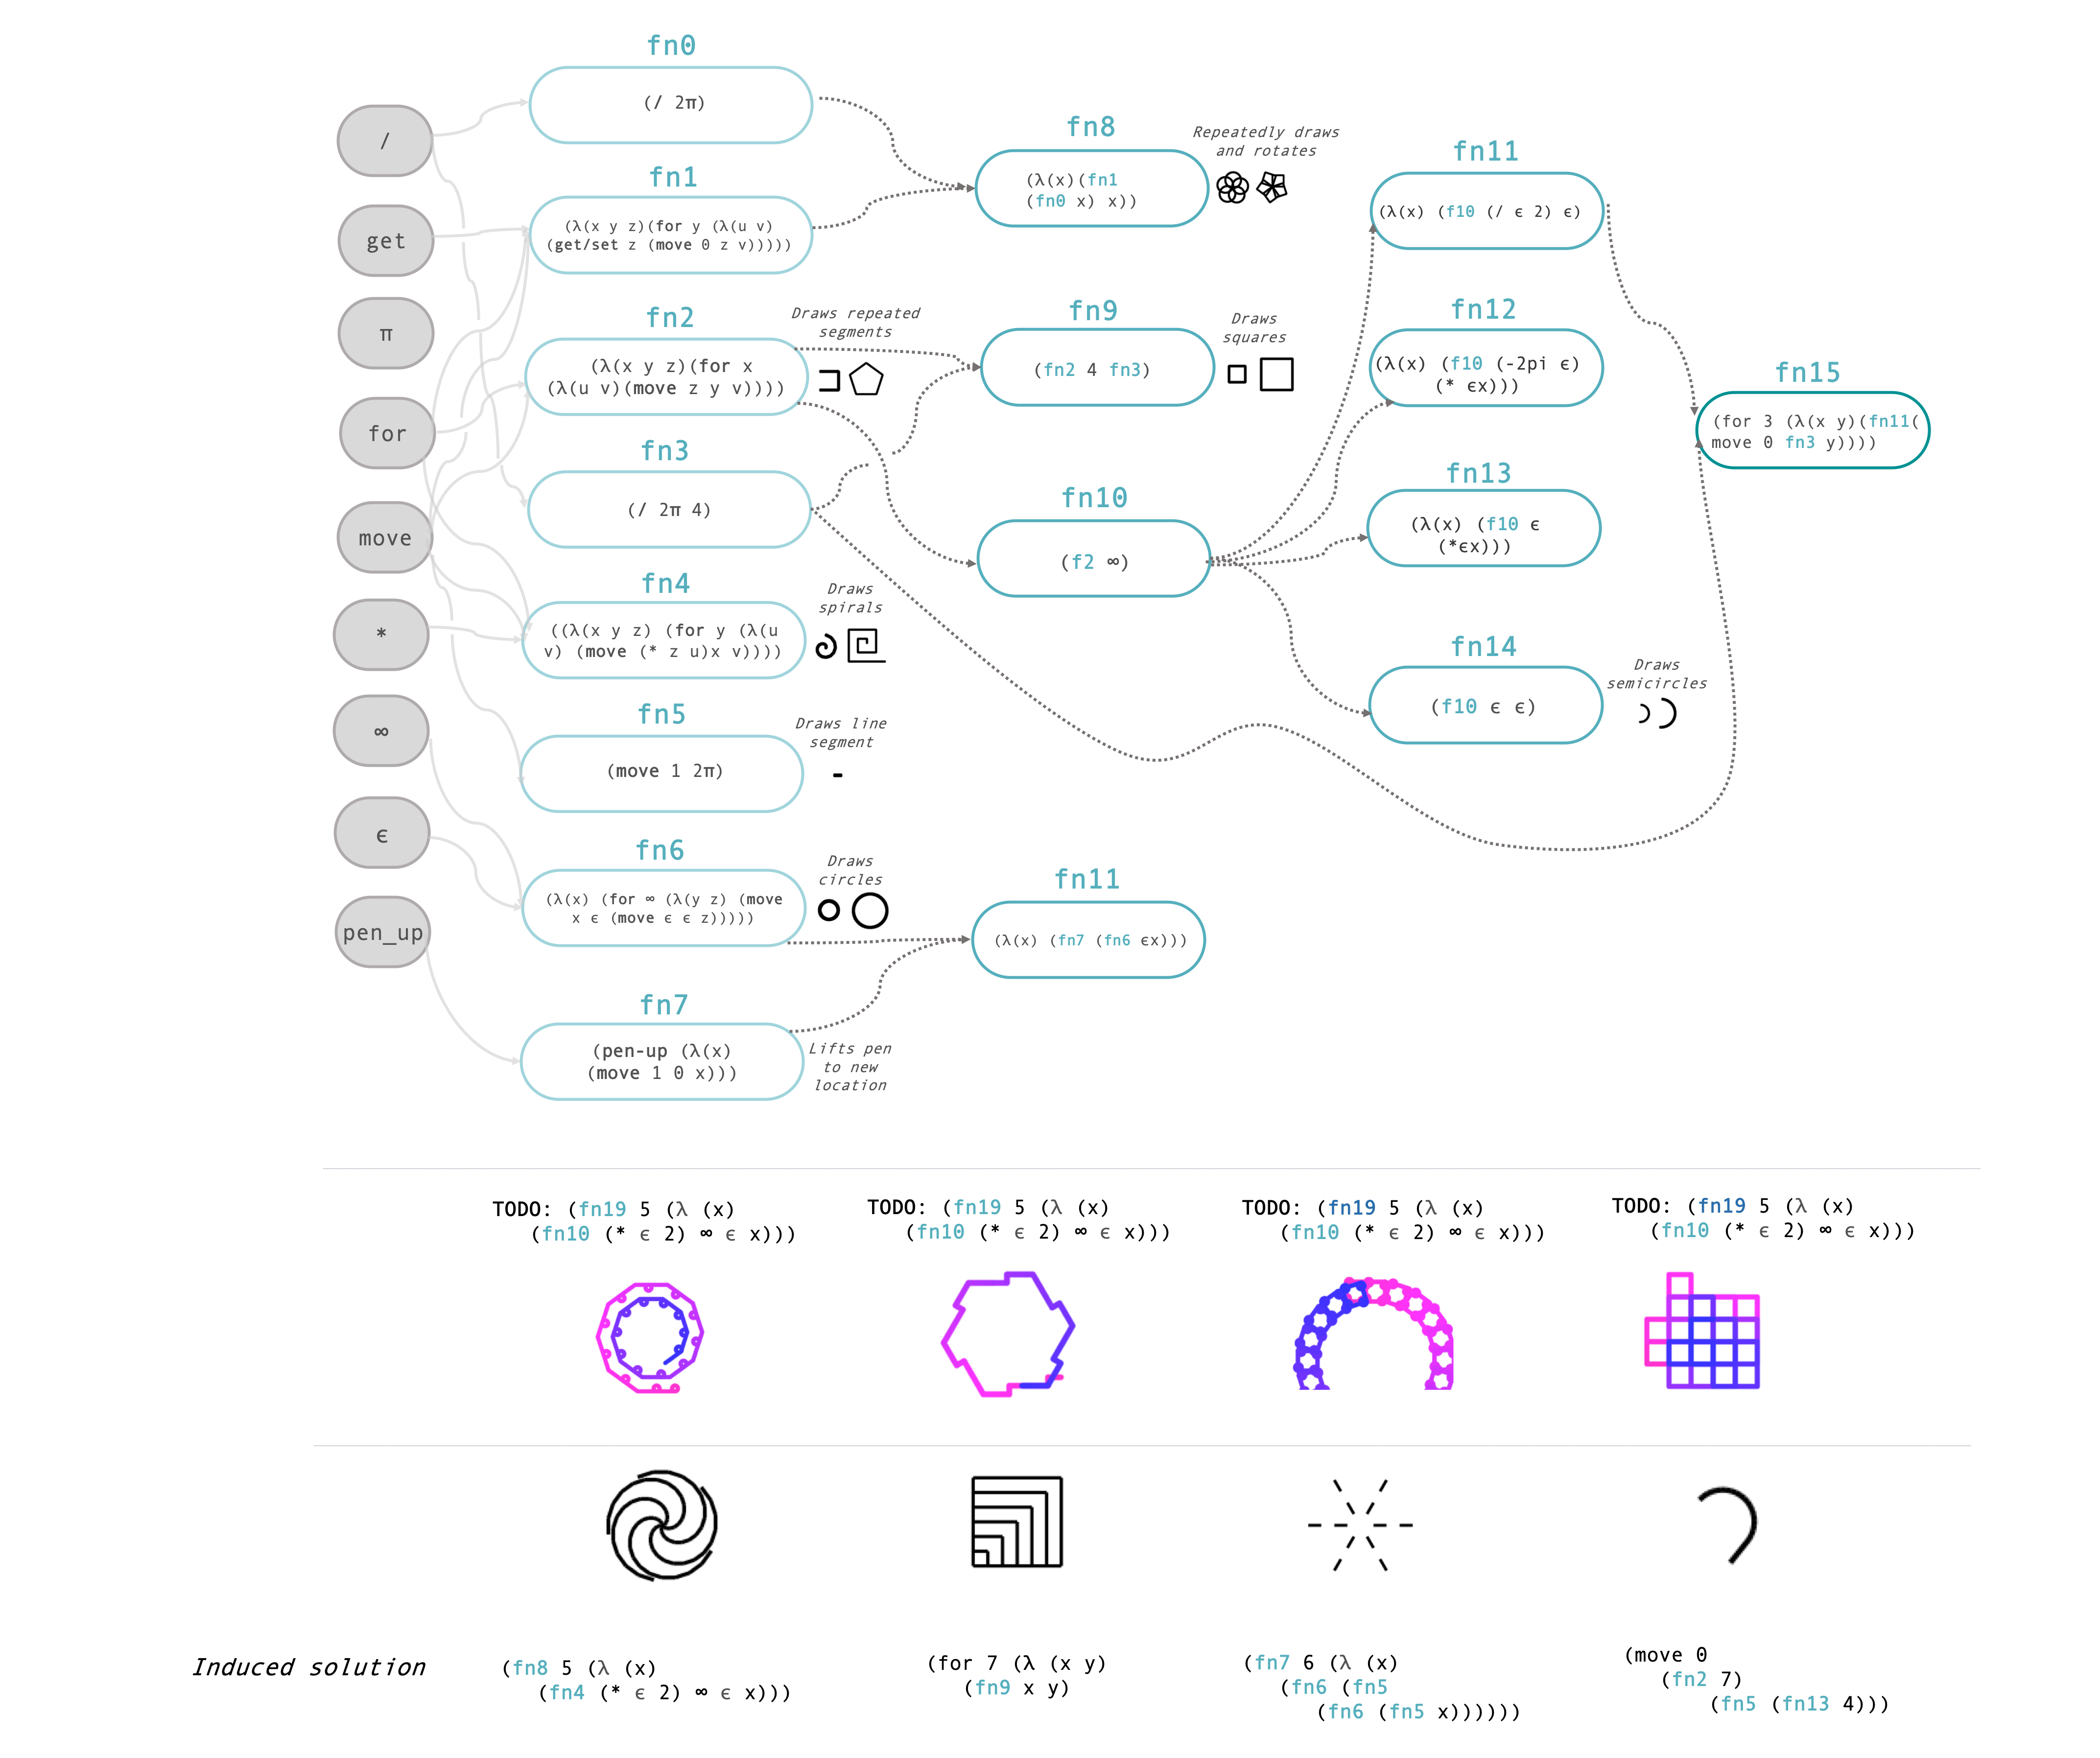
\includegraphics[width=0.4\linewidth]{logo.png} & \hfill & 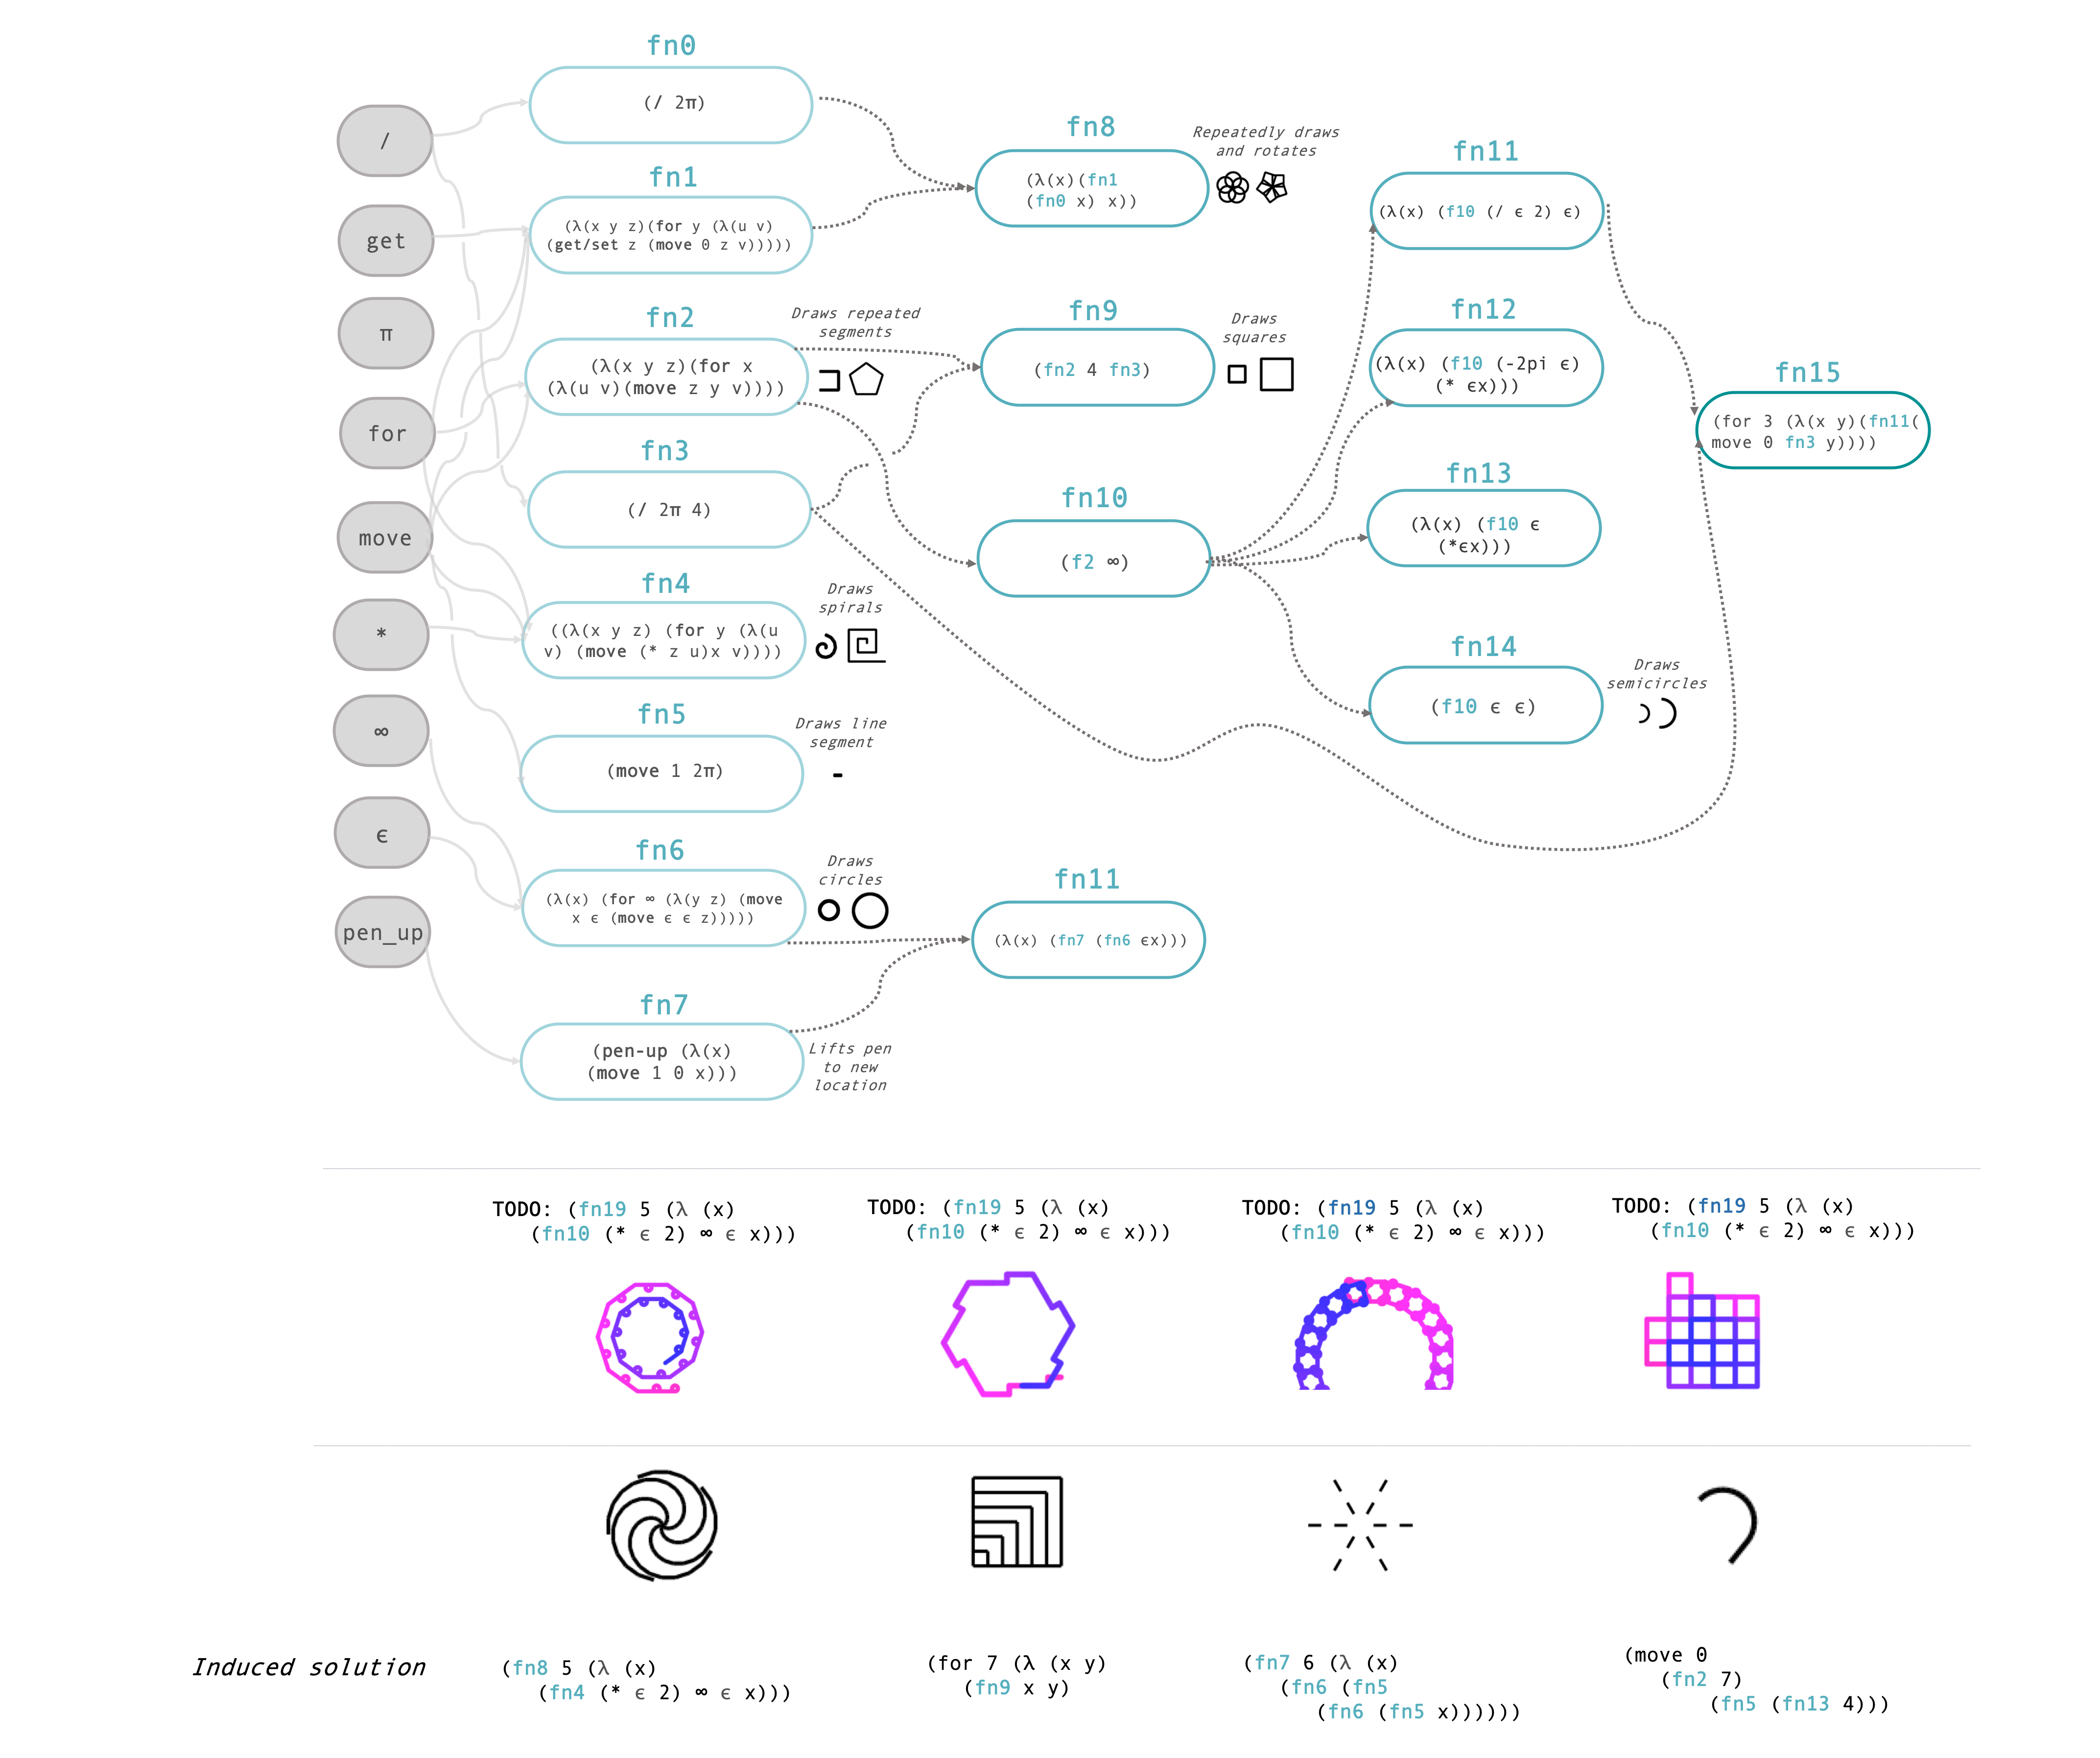
\includegraphics[width=0.4\linewidth]{logo.png}
%% \end{tabular}
%% \end{center}

%% %----------------------------------------------------------------------------------------

%% \end{column}
% End of the third column

\end{columns} % End of all the columns in the poster

\end{frame} % End of the enclosing frame

\end{document}
